\documentclass{article}
\usepackage{lipsum}
\usepackage{amsmath}
\usepackage{graphicx}
\usepackage{subcaption}
\usepackage{biblatex}

\title{Final Project}
\author{Amir Hasanshahi}
\date{December 22, 2024}

\addbibresource{references.bib}

\begin{document}
	\maketitle
	\tableofcontents
	\newpage

	\section{Introduction}
	\lipsum[1-3]
	\newpage

	\section{Source of information}
	\subsection{Equations}
	\begin{align}
		p(x) & = x^{4}- 2x^{3}+ 5x - 8 \\
		q(x) & = 3x^{2}- 7x + 2
	\end{align}
	\begin{equation*}
		J(\theta) = \frac{1}{m}\left[-y^{(i)}\log(h_{\theta}(x^{(i)})) -(1 - y^{(i)})
		\log(1-h_{\theta}(x(i)))\right] + \frac{\lambda}{2m}\sum_{j = 1}^{n}(\theta )
		_{j}^{2}
	\end{equation*}
	\subsection{Images}
	\begin{figure*}[ht]
		\centering
		
\includegraphics[width=0.5\textwidth]{rb_20368.png}
		\caption{flowers}
		\label{flowres}
	\end{figure*}
	\begin{figure*}[ht]
		\centering
		\begin{subfigure}
			{0.45\textwidth}
			\centering
			
\includegraphics[width=\textwidth]{rb_154283.png}
			\caption{davy jones}
			\label{davy jones}
		\end{subfigure}
		\begin{subfigure}
			{0.45\textwidth}
			\centering
			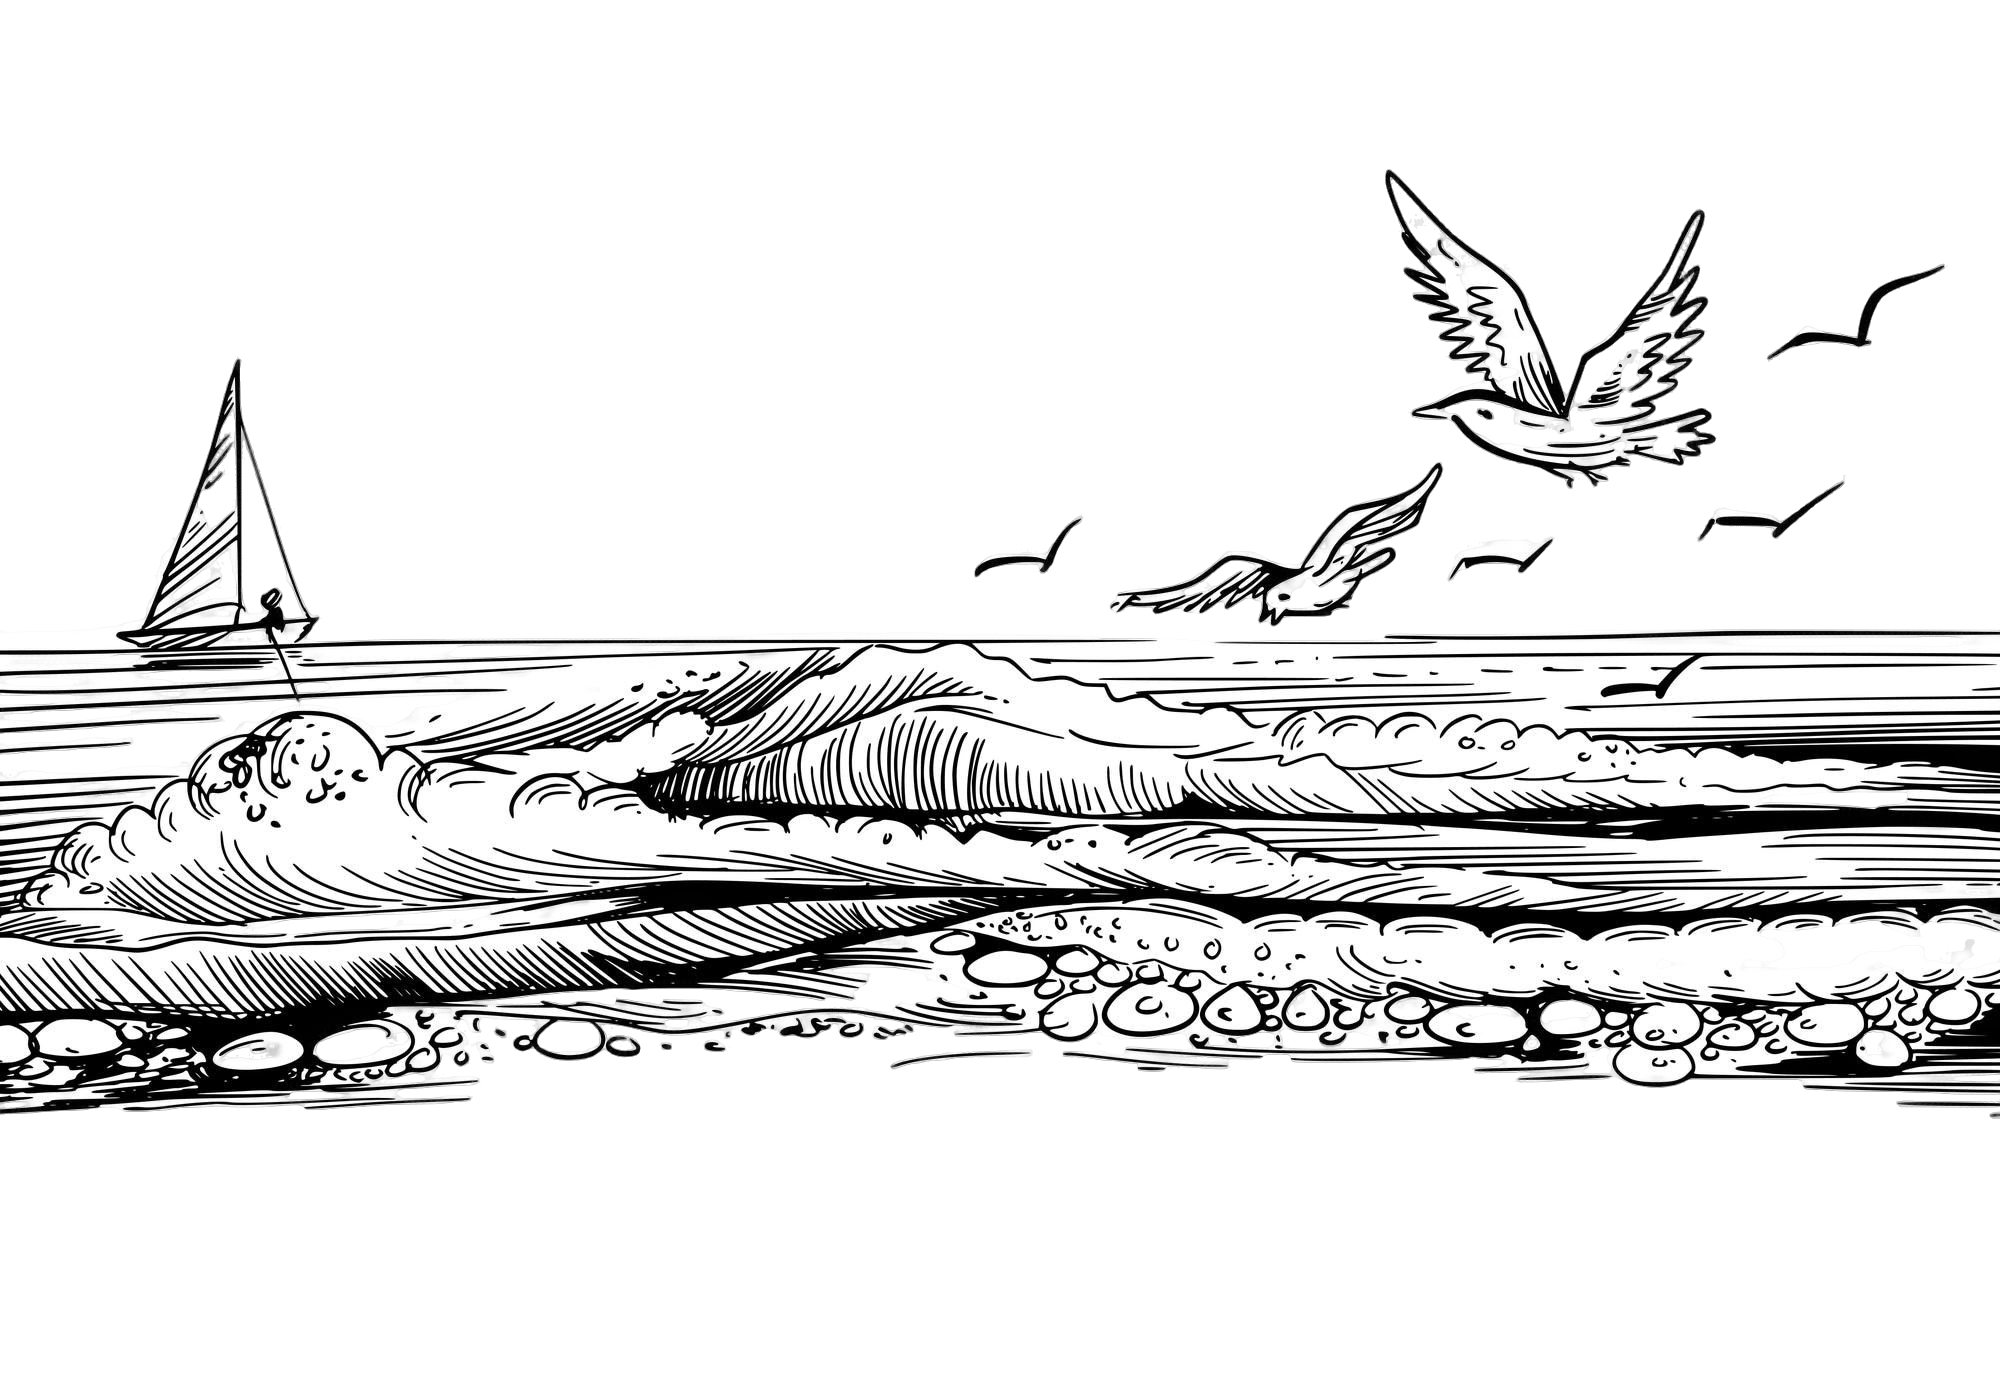
\includegraphics[width=\textwidth]{rb_28519.png}
			\caption{sea}
			\label{sea}
		\end{subfigure}
		\hfil
	\end{figure*}
	\newpage
	\subsection{Table of data}
	\begin{table}[h]
		\centering
		\begin{tabular}{|c|c|c|}
			\hline
			     & height (m) & weight (kg) \\
			\hline
			John & 1.68       & 60          \\
			\hline
			Wick & 1.92       & 80          \\
			\hline
		\end{tabular}
		\caption{table}
		\label{table}
	\end{table}

	\section{Ending}
	\textit{This article is written by \textbf{\citeauthor{FinalArticle}} in \textbf{\citedate{FinalArticle}}}

	\printbibliography
\end{document}